\definecolor{purple}{rgb}{0.65, 0.12, 0.82}
\definecolor{superlightgrey}{rgb}{217,217,217}
\lstdefinelanguage{JavaScript}{
  keywords={break, case, catch, continue, debugger, default, delete, do, else,
  false, finally, for, function, if, in, instanceof, new, null, return, switch,
  this, throw, true, try, typeof, var, void, while, with}, morecomment=[l]{//},
  morecomment=[s]{/*}{*/}, morestring=[b]', morestring=[b]", ndkeywords={class,
  export, boolean, throw, implements, import, this},
  keywordstyle=\color{blue}\bfseries, ndkeywordstyle=\color{darkgray}\bfseries,
  identifierstyle=\color{black}, commentstyle=\color{purple}\ttfamily,
  stringstyle=\color{red}\ttfamily, sensitive=true,    breaklines=true,
    frame=lines
}

\lstset{
   language=JavaScript, backgroundcolor=\color{superlightgrey},
   extendedchars=true, basicstyle=\footnotesize\ttfamily,
   showstringspaces=false, showspaces=false, numbers=left,
   numberstyle=\footnotesize, numbersep=9pt, tabsize=2, breaklines=true,
   showtabs=false, captionpos=b
}

\chapter{Software Architecture}
\section{Requirements}
\label{sec:Requirements} 

\section{Implementation}
\label{Implementation}

\subsection{Actual Setup}
\label{setup}


\newpage
\subsection{WebSockets}

\begin{figure}[ht]
	\centering
	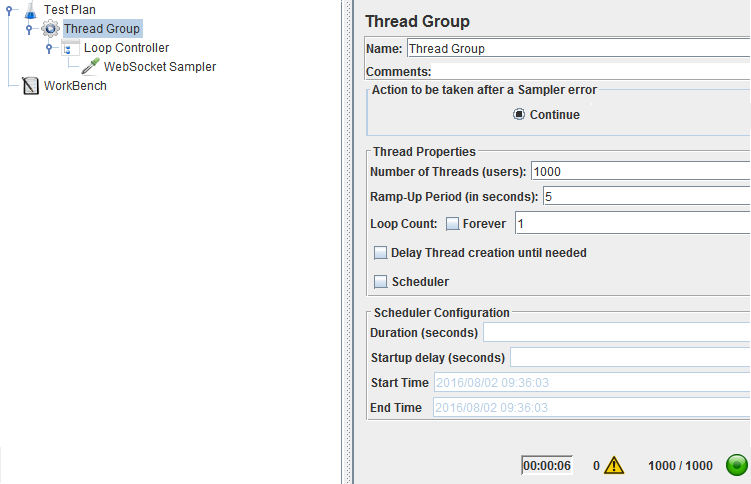
\includegraphics[scale=0.7]{Bilder/jMeterReal.png}
	 \caption[Testing with jMeter]{jMeter testing}
  	\label{fig:testing}
\end{figure}


